\chapter{Other SUSY results}
\label{chap:summary_susy}

In this chapter we discuss the interplay of the searched presented in the previous two chapters and the 
wide program of \gls{susy} searched carried on by the \gls{atlas} and \gls{cms} collaborations. 

\section{Gluino pair production}


\section{RPV interpretation}


\section{Higgsino pair production in GMSB models}

\begin{figure}[htbp]
	\centering
	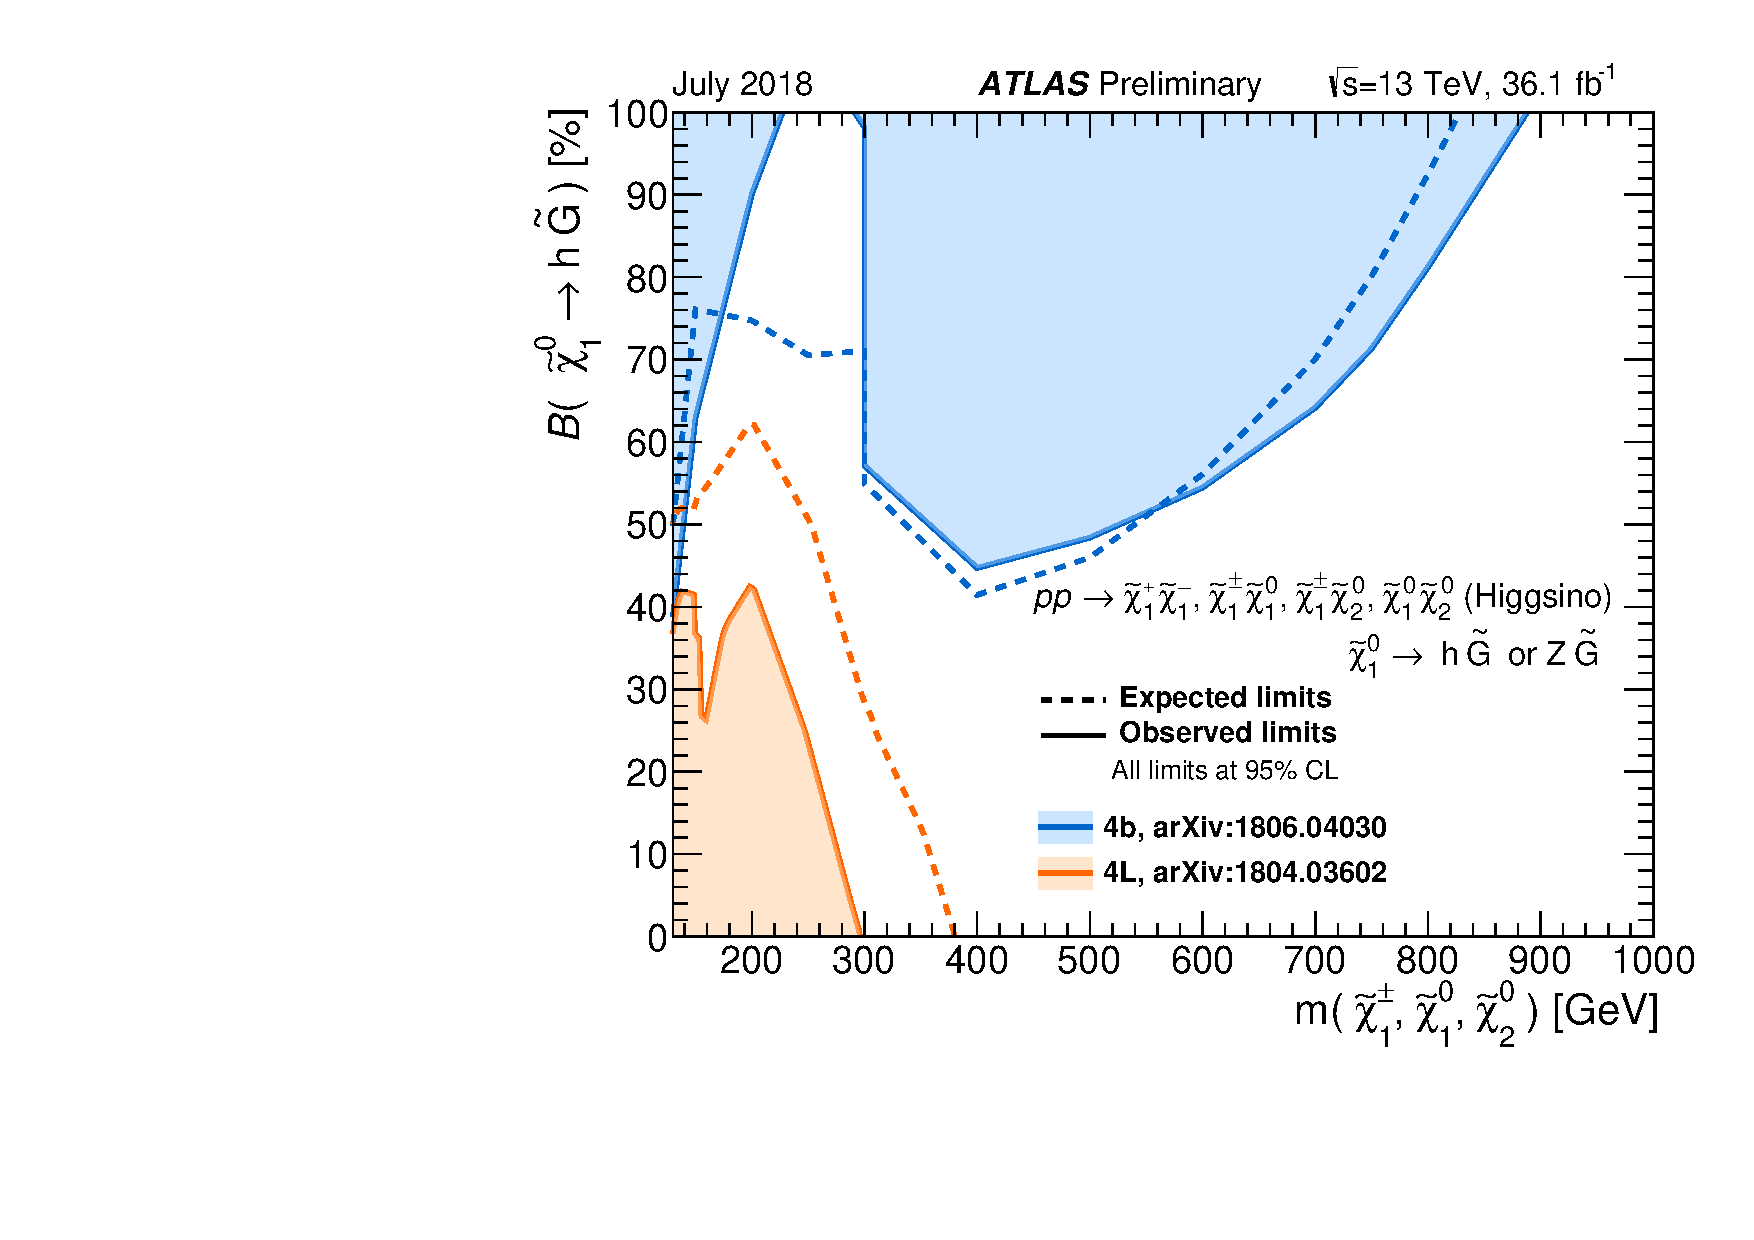
\includegraphics[width=0.75\textwidth]{figures/summary_plots/ATLAS_SUSY_EWSummary_GGM.pdf}
	\caption{The 95\% CL exclusion limits on a general gauge mediation model from 13 TeV data. 
	The model assumes a pure Higgsino NLSP that promptly decays to either Z gravitino or Higgs gravitino. 
	The limits are displayed as a function of the mass of the nearly mass-degenerate Higgsino triplet and the branching fraction of lightest Higgsino to Higgs gravitino. 	
	} 
	\label{fig:summary_higgsino_GMSB}
\end{figure}

